\documentclass{beamer}
\usecolortheme{dove}
\setbeamertemplate{navigation symbols}{}
\usepackage{amsmath,amssymb,amsfonts,amsthm, multicol, subfigure, color}
\usepackage{bm}
\usepackage{graphicx}
\usepackage{tabularx}
\usepackage{booktabs}
\usepackage{hyperref}
\usepackage{pdfpages}
\usepackage{xcolor}
\definecolor{seagreen}{RGB}{46, 139, 87}
\definecolor{ucla}{RGB}{39, 116, 174}
\definecolor{darkestblue}{RGB}{0, 59, 92}
\definecolor{gold}{RGB}{255, 209, 0}
\def\independenT#1#2{\mathrel{\rlap{$#1#2$}\mkern2mu{#1#2}}}
\newcommand\indep{\protect\mathpalette{\protect\independenT}{\perp}}
\def\log{\text{log}}
\newcommand\logit{\text{logit}}
\newcommand\iid{\stackrel{\text{iid}}{\sim}}
\newcommand\E{\text{E}}
\newcommand\V{\text{V}}
\renewcommand\P{\text{P}}
\newcommand{\Cov}{\text{Cov}}
\newcommand{\Cor}{\text{Cor}}
\newcommand\doop{\text{do}}


\usepackage{stackrel}
\usepackage{tikz}
\usetikzlibrary{arrows,shapes.arrows,positioning,shapes,patterns,calc}
\newcommand\slideref[1]{\vskip .1cm \tiny \textcolor{gray}{{#1}}}
\newcommand\red[1]{\color{red}#1}
\newcommand\blue[1]{\color{blue}#1}
\newcommand\gray[1]{\color{gray}#1}
\newcommand\seagreen[1]{\color{seagreen}#1}
\newcommand\purple[1]{\color{purple}#1}
\newcommand\orange[1]{\color{orange}#1}
\newcommand\black[1]{\color{black}#1}
\newcommand\white[1]{\color{white}#1}
\newcommand\teal[1]{\color{teal}#1}
\newcommand\magenta[1]{\color{magenta}#1}
\newcommand\Fuchsia[1]{\color{Fuchsia}#1}
\newcommand\BlueGreen[1]{\color{BlueGreen}#1}
\newcommand\bblue[1]{\textcolor{blue}{\textbf{#1}}}
\newcommand\bred[1]{\textcolor{red}{\textbf{#1}}}
\newcommand\bgray[1]{\textcolor{gray}{\textbf{#1}}}
\newcommand\bgreen[1]{\textcolor{seagreen}{\textbf{#1}}}
\newcommand\bref[2]{\href{#1}{\color{blue}{#2}}}
\colorlet{lightgray}{gray!40}
\pgfdeclarelayer{bg}    % declare background layer for tikz
\pgfsetlayers{bg,main} % order layers for tikz
\newcommand\mycite[1]{\begin{scriptsize}\textcolor{darkgray}{(#1)}\end{scriptsize}}
\newcommand{\tcframe}{\frame{
%\small{
\only<1|handout:0>{\tableofcontents}
\only<2|handout:1>{\tableofcontents[currentsection]}}
%}
}

\setbeamertemplate{footline}[frame number]


\usepackage[round]{natbib}
\bibliographystyle{humannat-mod}
\setbeamertemplate{enumerate items}[default]
\usepackage{mathtools}

\newcommand{\goalsframe}{\begin{frame}{Learning goals for today}
At the end of class, you will be able to:
\begin{enumerate}
\item Read a Directed Acyclic Graph
\item Recognize causal paths
\item Understand two key structures
\begin{itemize}
\item Fork structures ($\bullet\leftarrow\bullet\rightarrow\bullet$)
\item Collider structures ($\bullet\rightarrow\bullet\leftarrow\bullet$)
\end{itemize}
\item List all paths in a DAG
\item Determine which paths are blocked under a particular adjustment set
\item Select a sufficient adjustment set to isolate causal paths
\end{enumerate} \vskip .2in
\end{frame}}

\title{Directed Acyclic Graphs}
\author{Sociol 114}
\date{6 Feb 2025}

\begin{document}

\maketitle

\goalsframe

\begin{frame}
\includegraphics[width = \textwidth]{figures/conditional_randomization} \\
Outcome: Employed at age 40

\end{frame}

\begin{frame}[t]{Elements of a Directed Acyclic Graph (DAG)}

\begin{center}
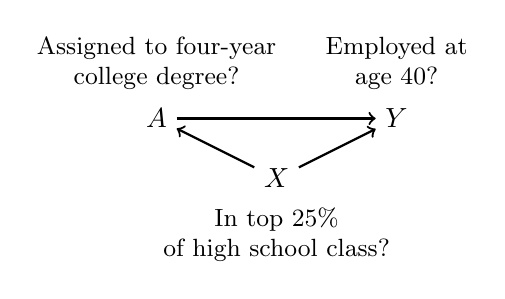
\begin{tikzpicture}[x = .3in, y = .3in]
    \node at (-3,0) {};
    \node at (3,0) {};
    \node (x) at (0,-1) {$X$};
    \node (a) at (-2,0) {$A$};
    \node (y) at (2,0) {$Y$};
    \draw[->, thick] (x) -- (a);
    \draw[->, thick] (a) -- (y);
    \draw[->, thick] (x) -- (y);
        % Labels
    \node[anchor = north, font = \small, align = center] at (x.south) {In top 25\%\\of high school class?};
    \node[anchor = south, font = \small, align = center] at (a.north) {Assigned to four-year\\college degree?};
    \node[anchor = south, font = \small, align = center] at (y.north) {Employed at\\age 40?};
  \end{tikzpicture}
\end{center}
  
  \begin{itemize}
  \item \textbf{Nodes} ($X,A,Y$) are random variables
  \item \textbf{Edges} ($\rightarrow$) are causal relationships.
  \begin{itemize}
  \item $X$ has a causal effect on $A$
  \item $X$ has a causal effect on $Y$
  \item $A$ has a causal effect on $Y$
  \end{itemize}
  \end{itemize}
  
\end{frame}

\begin{frame}[t]{Elements of a Directed Acyclic Graph (DAG)}

\begin{center}
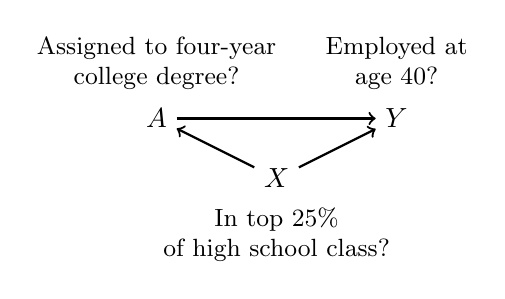
\begin{tikzpicture}[x = .3in, y = .3in]
    \node at (-3,0) {};
    \node at (3,0) {};
    \node (x) at (0,-1) {$X$};
    \node (a) at (-2,0) {$A$};
    \node (y) at (2,0) {$Y$};
    \draw[->, thick] (x) -- (a);
    \draw[->, thick] (a) -- (y);
    \draw[->, thick] (x) -- (y);
        % Labels
    \node[anchor = north, font = \small, align = center] at (x.south) {In top 25\%\\of high school class?};
    \node[anchor = south, font = \small, align = center] at (a.north) {Assigned to four-year\\college degree?};
    \node[anchor = south, font = \small, align = center] at (y.north) {Employed at\\age 40?};
  \end{tikzpicture}
\end{center}

A \textbf{path} is a sequence of edges connecting two nodes. \vskip .1in \pause
Between $A$ and $Y$, what are the two paths? \pause
\begin{itemize}
\item $A\rightarrow Y$
\item $A\leftarrow X \rightarrow Y$
\end{itemize}

\end{frame}

\begin{frame}{Causal paths}

In a \textbf{causal path}, all arrows point in the same direction.\\($\bullet\rightarrow\bullet\rightarrow\bullet$) \vskip .2in \pause

What three paths between $A$ and $Y$? \\
Which two are causal paths? \\

\begin{center}
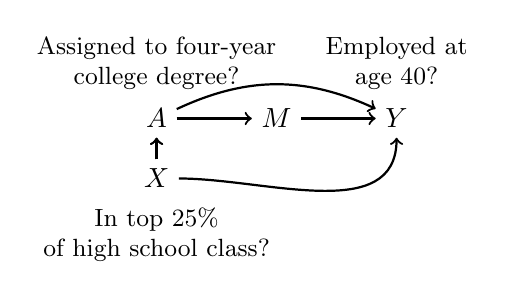
\begin{tikzpicture}[x = .3in, y = .3in]
    \node at (-3,0) {};
    \node at (3,0) {};
    \node (x) at (-2,-1) {$X$};
    \node (a) at (-2,0) {$A$};
    \node (m) at (0,0) {$M$};
    \node (y) at (2,0) {$Y$};
    \draw[->, thick] (x) -- (a);
    \draw[->, thick] (a) to[bend left = 25] (y);
    \draw[->, thick] (a) -- (m);
    \draw[->, thick] (m) -- (y);
    \draw[->, thick] (x) -- (a);
    \draw[->, thick] (x) to[out = 0, in = 270] (y);
        % Labels
    \node[anchor = north, font = \small, align = center] at (x.south) {In top 25\%\\of high school class?};
    \node[anchor = south, font = \small, align = center] at (a.north) {Assigned to four-year\\college degree?};
    \node[anchor = south, font = \small, align = center] at (y.north) {Employed at\\age 40?};
  \end{tikzpicture}
\end{center} \pause \vskip .1in
\begin{tabular}{ll}
$A\rightarrow Y$ & \only<4->{causal path} \\
$A\rightarrow M \rightarrow Y$ & \only<5->{causal path} \\
$A\leftarrow X \rightarrow Y$ & \only<6->{not a causal path}
\end{tabular}

\end{frame}

\begin{frame}{Causal paths}

When two variables are connected by a causal path, those variables are statistically associated (because the first variable causes the second) unless you hold constant some variable along the path \vskip .2in \pause

Example: Among people with a fever,\\
($A$: friend offers Tylenol) $\rightarrow$ ($M$: person takes Tylenol)\\$\rightarrow$ ($Y$: Fever subsides quickly)
\begin{itemize}
\item Marginally, this causal path makes $A$ associated with $Y$
\begin{itemize}
\item Fevers subsided more quickly among those whose friend offered Tylenol
\end{itemize}
\item Conditional on $M = 0$, $A$ and $Y$ are unrelated
\begin{itemize}
\item Among those who didn't take Tylenol, it doesn't matter whether a friend offered them Tylenol or not. Fevers were the same.
\end{itemize}
\end{itemize}

\end{frame}

\begin{frame}[t]{Fork structures}

A \textbf{fork structure} is a sequence of edges within a path in which two variables are both caused by a third variable: $A\leftarrow C \rightarrow B$ \pause \vskip .1in

In our initial graph, what path contains a fork structure?

\begin{center}
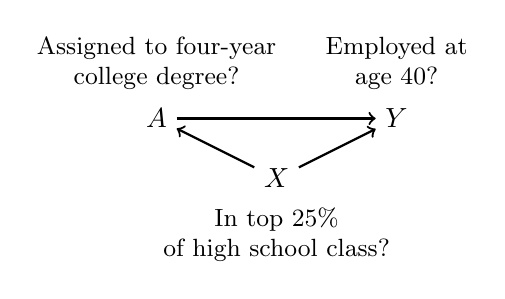
\begin{tikzpicture}[x = .3in, y = .3in]
    \node at (-3,0) {};
    \node at (3,0) {};
    \node (x) at (0,-1) {$X$};
    \node (a) at (-2,0) {$A$};
    \node (y) at (2,0) {$Y$};
    \draw[->, thick] (x) -- (a);
    \draw[->, thick] (a) -- (y);
    \draw[->, thick] (x) -- (y);
        % Labels
    \node[anchor = north, font = \small, align = center] at (x.south) {In top 25\%\\of high school class?};
    \node[anchor = south, font = \small, align = center] at (a.north) {Assigned to four-year\\college degree?};
    \node[anchor = south, font = \small, align = center] at (y.north) {Employed at\\age 40?};
  \end{tikzpicture}
\end{center}

Recall that there are two paths:
\begin{enumerate}
\item $A\rightarrow Y$
\item $A\leftarrow X \rightarrow Y$ \onslide<3->{(this path contains a fork structure)}
\end{enumerate}



\end{frame}


\goalsframe

\end{document}

